% !TEX TS-program = pdflatexmk

\documentclass[14pt]{beamer}
\usepackage{newtxtext,newtxmath}
\usepackage{microtype}
\usepackage[english]{babel}
\usepackage{array}
\usepackage{booktabs}
\usepackage{graphicx}
\usepackage{tikz}
\usetikzlibrary{fit}
\usetikzlibrary{positioning}
\usetikzlibrary{shadows}
\usetikzlibrary{shapes}
\usetikzlibrary{shapes.multipart}


% Define UA colors
% https://brand.arizona.edu/applying-the-brand/colors
\definecolor{ua-red}{HTML}{AB0520}
\definecolor{ua-blue}{HTML}{0C234B}
\definecolor{ua-oasis}{HTML}{378DBD}

\mode<presentation>{
\usetheme{Madrid}
\usecolortheme[named=ua-red]{structure}
\setbeamertemplate{navigation symbols}{}
\setbeamertemplate{footline}[frame number]
\setbeamertemplate{section in toc}[square]
\setbeamertemplate{subsection in toc}[square]
\setbeamertemplate{items}[square]
\setbeamercovered{transparent=0}
}

\tikzset{
  doc/.style={
    draw, minimum height=3em, minimum width=2em, fill=white,
    double copy shadow={shadow xshift=-4pt, shadow yshift=-4pt, fill=white, draw}
  },
  ml model/.style={
    node contents={
\includegraphics[scale=#1]{Hey_Machine_Learning_Logo.png}},
    inner sep=0pt,
  },
  ml model/.default={1},
}

% command for annotating words in text
% #1: drawing options
% #2: name of entire shape
% #3: number of parts
% #4: name of baseline part
% #5: annotation type
% #6: node text following \nodepart{two}
\newcommand{\annotate}[6][]{%
\tikz[remember picture,baseline={(#2.#4)}]{%
\node[
  rectangle split,
  rectangle split parts=#3,
  thick,
  inner sep=2pt,
  align=center,
  draw,
  #1]%
(#2)
{%
\scriptsize\strut\textsc{#5}%
\nodepart{two}%
#6%
\strut};}}

\newcommand{\AnnotateTwo}[4][]{\annotate[#1]{#2}{2}{two}{#3}{#4}}


\author[Bethard]{Dr. Steven Bethard}
\institute[Arizona]{%
School of Information\\
University of Arizona}

\title{Adapting natural language processing models across clinical domains}
\date[]{26 Feb 2021}


\begin{document}


\begin{frame}
  \titlepage
\end{frame}

\section{Machine learning needs domain adaptation}

\begin{frame}{Machine learning needs adaptation}
\small
\begin{tikzpicture}[data/.style={font=\scriptsize}]

\node[data, label={[align=center, inner sep=0pt]Source Domain\\(large labeled data)}] (source-data) at (0, 2) {
\begin{tabular}{@{} l l @{}}
\toprule
Input & Output \\
\midrule
Dec 5, 2007 & 2007-12-05 \\
3 Jan 2018 & 2018-01-03 \\
04-25-1990 & 1990-04-25 \\
\ldots & \ldots \\
\bottomrule
\end{tabular}
};

\node (model) at (4, 2) [ml model, label={Learned Model}];

\draw[ultra thick, -latex]  (source-data)  -- (model);

\visible<2->{
\node[data, label={[align=center, inner sep=0pt]Target Domain\\(unlabeled data)}] (target-data) at (0, -2) {
\begin{tabular}{@{} p{9em} @{}}
\toprule
Input \\
\midrule
3 weeks postoperative \\
1 tablet q.i.d \\
75-year-old \\
\ldots \\
\bottomrule
\end{tabular}
};
}

\visible<3->{
\node[data] (output) at (8, -2) {
\begin{tabular}{@{} p{9em} @{}}
\toprule
Output \\
\midrule
??? \\
??? \\
??? \\
\ldots \\
\bottomrule
\end{tabular}
};

\draw[ultra thick, dotted, -latex]  (target-data.east)  -- (model.south)  -- (output.west);
}
\end{tikzpicture}
\end{frame}

\begin{frame}{Machine learning needs adaptation}
A sample of recent NLP models, trained on a source domain, and tested on a target domain:

\bigskip
\footnotesize
\begin{tabular}{ l l l l l }
\toprule
& \multicolumn{2}{c}{Source} & \multicolumn{2}{c}{Target} \\
\cmidrule(lr){2-3}\cmidrule(lr){4-5}
Task & Domain & Score & Domain & Score \\
\midrule
Sentences & Mayo Clinic & 94.9 A & BIDMC ICU & 31.8 A \\
Syntax trees & Wall Street Journal & 89 $F_1$ & Medline abstracts & 75 $F_1$ \\
Negations & Partners Healthcare & 93.6 $F_1$ & Mayo Clinic & 74.7 $F_1$ \\
Times & Mayo colon cancer & 80 $F_1$ & Mayo brain cancer & 59 $F_1$ \\
\ldots \\
\bottomrule
\end{tabular}

\centering
\smallskip
Full table in \cite{laparra:JAMIAOpen:2020}
\end{frame}

\begin{frame}{Domain adaptive machine learning}
\small
\begin{tikzpicture}[data/.style={font=\scriptsize}]

\node[data, label={Source Domain}] (source-data) at (0, 2) {
\begin{tabular}{@{} l l @{}}
\toprule
Input & Output \\
\midrule
Dec 5, 2007 & 2007-12-05 \\
3 Jan 2018 & 2018-01-03 \\
04-25-1990 & 1990-04-25 \\
\ldots & \ldots \\
\bottomrule
\end{tabular}
};

\node[data, label={Target Domain}] (target-data) at (0, -2) {
\begin{tabular}{@{} l l @{}}
\toprule
Input & \color{lightgray} Output\\
\midrule
1 week postop &  \color{lightgray} 2011-07-06 \\
2 tablets b.i.d. &  \color{lightgray} 2$\times$2$\times$P1D \\
40-year-old &  \color{lightgray} P40Y \\
\ldots \\
\bottomrule
\end{tabular}
};

\node (model) at (6, 2)  [ml model, label={Learned Model}];

\draw[ultra thick, -latex]  (source-data)  -- (model.west);
\draw[ultra thick, -latex]  (target-data)  -- (model.west);

\visible<2->{\node[data] (input) at (4, -2) {
\begin{tabular}{@{} p{9em} @{}}
\toprule
Input \\
\midrule
3 weeks postoperative \\
1 tablet q.i.d. \\
75-year-old \\
\ldots \\
\bottomrule
\end{tabular}
};

\node[data] (output) at (8, -2) {
\begin{tabular}{@{} p{9em} @{}}
\toprule
Output \\
\midrule
2011-07-20 \\
1$\times$4$\times$P1D \\
P70Y \\
\ldots \\
\bottomrule
\end{tabular}
};

\draw[ultra thick, dotted, -latex]  (input)  -- (model.south) -- (output);
}
\end{tikzpicture}
\end{frame}

\begin{frame}{Domain adaptation is hard}
New label distributions for known phrases
\begin{itemize}
\item E.g., the word \textit{day}
\begin{itemize}
\item in news text is 68\% \textsc{Period}, 32\% \textsc{Calendar-Interval}
\item in clinical text is 6\% \textsc{Period}, 94\% \textsc{Calendar-Interval}
\end{itemize}
\end{itemize}

\pause
\bigskip
New phrases for known concepts
\begin{itemize}
\item E.g., \textit{q.i.d} meaning \textit{4 times per day}
\end{itemize}

\pause
\bigskip
New concepts
\begin{itemize}
\item E.g., \textit{lean season} or \textit{tef season}
\end{itemize}
\end{frame}

\begin{frame}{Clinical domain adaptation is even harder}
\begin{itemize}
\item Doctors notes vary wildly in format, style, and word choice depending on both medical institution and medical specialty
\begin{itemize}
\item E.g., for years cTAKES assumed newlines ended sentences because this was true in the Mayo Clinic EMR
\end{itemize}
\pause
\item Data is hard to share, due to protected health information
\begin{itemize}
\item IRB approvals and data use agreements can be complex
\item Previously approved data cannot be distributed without sustained funding (e.g., the Mayo Clinic's THYME corpus)
\item Many annotated datasets will never leave their original institution in any form
\end{itemize}
\end{itemize}
\end{frame}

\begin{frame}{Outline}
    \tableofcontents
\end{frame}

\AtBeginSection[]
{
  \begin{frame}<beamer>{Outline}
    \tableofcontents[currentsection]
  \end{frame}
}

\section{Domain adaptation comes in many forms}

\begin{frame}{Taxonomy of domain adaptation}
\begin{tabular}{ l l l }
\toprule
Souce shares & Target has & Example approach \\
\midrule
\pause
Labeled text & Labeled text & Feature augmentation \\
\pause
Labeled text & Raw text & Self-training \\
\pause
Trained models & Labeled text & Fine-tuning \\
\pause
Trained models & Raw text & ??? \\
\bottomrule
\end{tabular}
\end{frame}

\begin{frame}{Feature augmentation \hfill\small e.g., \cite{daume-iii-2007-frustratingly}}
\begin{tikzpicture}[
  font=\small,
  data/.style={font=\footnotesize, inner sep=0pt},
]

\node[doc,label={Source Domain}] (source-docs) at (-4, 1.5) {+1};

\node[data] (source-features) at (0, 1.5) {
\setlength{\tabcolsep}{0.5em}
\begin{tabular}{@{} c >{\color{ua-red}}c >{\color{ua-oasis}}c c @{}}
\toprule
Features & Source & Target & Label \\
\midrule
0 1 0 0 & 0 1 0 0 & 0 0 0 0 & +1\\
1 0 1 0 & 1 0 1 0 & 0 0 0 0 & -1\\
\ldots \\
\bottomrule
\end{tabular}
};

\node[doc,label={Target Domain}] (target-docs) at (-4, -1.5) {-1};

\node[data] (target-features) at (0, -1.5) {
\setlength{\tabcolsep}{0.5em}
\begin{tabular}{@{} c >{\color{ua-red}}c >{\color{ua-oasis}}c c @{}}
\toprule
Features & Source & Target & Label \\
\midrule
1 1 1 0 & 0 0 0 0 & 1 1 1 0 & -1 \\
0 0 1 1 & 0 0 0 0 & 0 0 1 1 & +1 \\
\ldots \\
\bottomrule
\end{tabular}
};

\node (model) at (4.8, 0) [ml model=0.8, label={Learned Model}];

\draw[ultra thick, -latex]  (source-docs) -- (source-features);
\draw[ultra thick, -latex]  (source-features.east)  -- (model);
\draw[ultra thick, -latex]  (target-docs) -- (target-features);
\draw[ultra thick, -latex]  (target-features.east)  -- (model);

\end{tikzpicture}

Assumptions:
\begin{itemize}
\item Source shares labeled text
\item Target has (small amounts of) labeled text
\end{itemize}
\end{frame}

\begin{frame}{Self-training \hfill\small e.g., \cite{yarowsky-1995-unsupervised,ruder-plank-2018-strong}}
\begin{tikzpicture}[
  font=\small,
  data/.style={font=\footnotesize, inner sep=0pt},
]

\node[doc,label={Source Domain}] (source-docs) at (-2, 1.5) {+1};

\node[data,anchor=west] (source-features) at (0, 1.5) {
\setlength{\tabcolsep}{0.5em}
\begin{tabular}{@{} c c @{}}
\toprule
Features & Label \\
\midrule
0 1 0 0 & +1\\
1 0 1 0 & -1\\
\ldots \\
\bottomrule
\end{tabular}
};

\node (model) at (6, 1.5) [ml model=0.8, label={Learned Model}];

\draw[ultra thick, -latex]  (source-docs) -- (source-features);
\draw[ultra thick, -latex]  (source-features.east)  -- (model);

\node[doc,label={Target Domain}] (target-docs) at (-2, -1.5) {?};

\visible<2->{
\node[data,anchor=west] (target-features) at (0, -1.5) {
\setlength{\tabcolsep}{0.5em}
\begin{tabular}{@{} c @{}}
\toprule
Features  \\
\midrule
1 1 1 0 \\
0 0 1 1 \\
\ldots \\
\bottomrule
\end{tabular}
};

\draw[ultra thick, -latex]  (target-docs) -- (target-features);
\draw[ultra thick, -latex]  (target-features.north)  -- (model);
}

\visible<3->{
\node[data] (target-labels) at (2.5, -1.5) {
\setlength{\tabcolsep}{0.5em}
\begin{tabular}{@{} c @{}}
\toprule
Labels  \\
\midrule
+1 \\
+1 \\
\ldots \\
\bottomrule
\end{tabular}
};

\draw[ultra thick, -latex]  (model)  -- (target-labels.north);
}

\visible<4->{
\node (st-model) at (6, -1.5)  [ml model=0.8, label={Self-trained Model}];

\draw [draw, thick] (-0.3,-2.8) rectangle (3.4,2.8);
\draw[ultra thick, -latex]  (3.4, -1.5)  -- (st-model);
}
\end{tikzpicture}

\begin{columns}
\begin{column}{0.53\textwidth}
Assumptions:
\begin{itemize}
\item Source shares labeled text
\item Target has raw text
\end{itemize}
\end{column}
\begin{column}<5->{0.45\textwidth}
Dangers:
\begin{itemize}
\item Poor pseudo-labels
\end{itemize}
\end{column}
\end{columns}
\end{frame}


\begin{frame}{Fine-tuning \hfill\small e.g., \cite{yosinski:NIPS:2014,lee-etal-2018-transfer}}
\begin{tikzpicture}[
  font=\small,
  data/.style={font=\footnotesize, inner sep=0pt},
]

\node[doc,label={Source Domain}] (source-docs) at (-2, 1.4) {+1};

\node[data,anchor=west] (source-features) at (0, 1.4) {
\setlength{\tabcolsep}{0.5em}
\begin{tabular}{@{} c c @{}}
\toprule
Features & Label \\
\midrule
0 1 0 0 & +1\\
1 0 1 0 & -1\\
\ldots \\
\bottomrule
\end{tabular}
};

\node (model) at (6, 1.4)  [ml model=0.8, label={Learned Model}];

\draw[ultra thick, -latex]  (source-docs) -- (source-features);
\draw[ultra thick, -latex]  (source-features.east)  -- (model);

\visible<2->{
\node[doc,label={Target Domain}] (target-docs) at (-2, -1.4) {-1};

\node[data,anchor=west] (target-features) at (0, -1.4) {
\setlength{\tabcolsep}{0.5em}
\begin{tabular}{@{} c c @{}}
\toprule
Features & Label \\
\midrule
1 1 1 0 & -1 \\
0 0 1 1 & +1\\
\ldots \\
\bottomrule
\end{tabular}
};

\draw[ultra thick, -latex]  (target-docs) -- (target-features);

\node (ft-model) at (6, -1.4) [ml model=0.8, label=below:{Fine-tuned Model}];

\draw[ultra thick, -latex]  (model)  -- (ft-model);
\draw[ultra thick, -latex]  (target-features)  -- (ft-model);
}
\end{tikzpicture}

\begin{columns}
\begin{column}{0.46\textwidth}
Assumptions:
\begin{itemize}
\item Source shares model
\item Target has labeled text
\end{itemize}
\end{column}
\begin{column}<3->{0.53\textwidth}
Dangers:
\begin{itemize}
\item Catastrophic forgetting \small\cite{mccloskey:PLM:1989}
\end{itemize}
\end{column}
\end{columns}
\end{frame}

\section{Domain adaptation for clinical information extraction}

\begin{frame}{SemEval-2021 Task 10}{Source-Free Domain Adaptation for Semantic Processing}
\begin{tikzpicture}[
  font=\small,
  data/.style={font=\footnotesize, inner sep=0pt},
]

\node[doc,label={Source Domain}] (source-docs) at (-3, 1.4) {+1};

\node[data] (source-features) at (0, 1.4) {
\setlength{\tabcolsep}{0.5em}
\begin{tabular}{@{} c c @{}}
\toprule
Features & Label \\
\midrule
0 1 0 0 & +1\\
1 0 1 0 & -1\\
\ldots \\
\bottomrule
\end{tabular}
};

\node (provided-model) at (3.5, 1.4)  [ml model=0.8, label={Provided Model}];

\draw[ultra thick, -latex]  (source-docs) -- (source-features);
\draw[ultra thick, -latex]  (source-features.east)  -- (provided-model);

\node[doc,label={Target Domain}] (target-docs) at (-3, -1.4) {?};

\node[draw,cloud,aspect=2,ua-red,ultra thick] (participant) at (0, -1.4) {Participant};

\draw[ultra thick, -latex]  (target-docs) -- (participant);
\draw[ultra thick, -latex]  (provided-model) -- (participant);

\node (adapted-model) at (3.5, -1.4)  [ml model=0.8, label={Adapted Model}];

\draw[ultra thick, -latex]  (participant) -- (adapted-model);

\node[data,anchor=west] (target-labels) at (5.5, -1.4) {
\setlength{\tabcolsep}{0.5em}
\begin{tabular}{@{} c @{}}
\toprule
Label \\
\midrule
-1 \\
+1\\
\ldots \\
\bottomrule
\end{tabular}
};

\draw[ultra thick, -latex]  (adapted-model) -- (target-labels);
\end{tikzpicture}
\end{frame}

\begin{frame}{SemEval-2021 Task 10}{Source-Free Domain Adaptation for Semantic Processing}
\begin{columns}
\begin{column}{0.45\textwidth}
\begin{block}{Task: Negation}
\small
Has frequent \AnnotateTwo{diarrhea}{}{diarrhea}, but no new \AnnotateTwo{lumps}{Negated}{lumps} or \AnnotateTwo{masses}{Negated}{masses}\ldots
\end{block}
\end{column}
\begin{column}{0.5\textwidth}
\begin{block}{Task: Time Expressions}
\small
In \AnnotateTwo{month}{Month-Of-Year}{January} of \AnnotateTwo{year}{Year}{2009}, she had pain \AnnotateTwo{number}{Number}{four} \AnnotateTwo{period}{Period}{hours} \AnnotateTwo{after}{After}{after}\ldots
\end{block}
\end{column}
\end{columns}

\pause
\bigskip
\small
\begin{tabular}{@{} l l l @{}}
\toprule
& Negation & Time Expressions  \\
\midrule
Trained model & Mayo Clinic (10K) & Mayo Clinic (18K) \\
Dev data & Partners HealthCare (5K) & News (2K) \\
Test data & Beth Israel ICU (9K) & Food Insecurity (2K) \\
\bottomrule
\end{tabular}
\end{frame}

\begin{frame}{SemEval-2021 Task 10}{Source-Free Domain Adaptation for Semantic Processing}


\begin{tabular}{ l c c c c c c }
\toprule
& \multicolumn{3}{c}{Negation} & \multicolumn{3}{c}{Time Expressions} \\
\cmidrule(lr){2-4}\cmidrule(lr){5-7}
System & P & R & $F_1$ & P & R & $F_1$ \\
\midrule
Provided model & 91.7 & 51.6 & \alert<2>{66.0} & 84.9 & 74.6 & \alert<2>{79.4} \\
Fine-tune on dev & 90.8 & 61.1 & \alert<2-3>{73.0} & 82.7 & 78.2 & \alert<2-3>{80.4} \\
Top participant & 90.2 & 75.6 & \alert<3>{82.2} & 84.7 & 78.5 & \alert<3>{81.5} \\
\bottomrule
\end{tabular}

\bigskip
Findings:
\begin{itemize}
\item<2-> Fine-tuning on dev domain helps; no catastrophic forgetting, and despite test domain being different
\item<3-> Participant systems made larger gains on negation than time expressions
\end{itemize}
\end{frame}

\begin{frame}{Source-free self-trained fine-tuning}
\begin{tikzpicture}[
  font=\small,
  data/.style={font=\footnotesize, inner sep=0pt},
]

\node (provided-model) at (1.5, 1.5) [ml model=0.8, label={Provided Model}];

\node[doc,label={Target Domain}] (target-docs) at (-2, -1.5) {?};

\node[data,anchor=west] (target-features) at (0, -1.5) {
\setlength{\tabcolsep}{0.5em}
\begin{tabular}{@{} c @{}}
\toprule
Features  \\
\midrule
1 1 1 0 \\
0 0 1 1 \\
\ldots \\
\bottomrule
\end{tabular}
};

\draw[ultra thick, -latex]  (target-docs) -- (target-features);
\draw[ultra thick, -latex]  (target-features.north)  -- (provided-model.south);

\node[data] (target-labels) at (2.5, -1.5) {
\setlength{\tabcolsep}{0.5em}
\begin{tabular}{@{} c @{}}
\toprule
Labels  \\
\midrule
+1 \\
+1 \\
\ldots \\
\bottomrule
\end{tabular}
};

\draw[ultra thick, -latex]  (provided-model.south)  -- (target-labels.north);

\visible<2->{
\node (st-model) at (6, -1.5)  [ml model=0.8, label={Adapted Model}];

\draw[ultra thick, -latex]  (provided-model)  -- (st-model);
\draw[ultra thick, -latex]  (target-labels)  -- (st-model);
}
\end{tikzpicture}

\bigskip
\onslide<3->
Results:
\begin{itemize}
\item +4.7 $F_1$ on negation (rank 2)
\item no gain on time expressions
\end{itemize}
\end{frame}


\begin{frame}{Source-free active-learned fine-tuning}
\begin{tikzpicture}[
  font=\small,
  data/.style={font=\footnotesize, inner sep=0pt},
]

\node (provided-model) at (4, 1.35) [ml model=0.8, label={Provided Model}];

\node[doc,label={Target Domain}] (target-docs) at (-2, 1.35) {?};

\node (human) at (-2, -1.35)  {
\includegraphics[scale=0.5]{female-user.pdf}};

\draw[ultra thick, -latex,align=center]  (target-docs) --  node[auto,swap,pos=0.8] {Select $k$ \\ by entropy} (human);

\node[data,anchor=west] (target-features) at (0, 1.35) {
\setlength{\tabcolsep}{0.5em}
\begin{tabular}{@{} c @{}}
\toprule
Features  \\
\midrule
1 1 1 0 \\
0 0 1 1 \\
\ldots \\
\bottomrule
\end{tabular}
};

\draw[ultra thick, -latex]  (target-docs) -- (target-features);

\node[data,anchor=west] (target-labels) at (0, -1.35) {
\setlength{\tabcolsep}{0.5em}
\begin{tabular}{@{} c @{}}
\toprule
Labels  \\
\midrule
+1 \\
+1 \\
\ldots \\
\bottomrule
\end{tabular}
};

\draw[ultra thick, -latex]  (human) -- (target-labels);

\visible<2->{
\node (st-model) at (4, -1.35)  [ml model=0.8, label=below:{Adapted Model}];

\draw[ultra thick, -latex]  (provided-model)  -- (st-model);
\draw[ultra thick, -latex]  (target-features)  -- (st-model);
\draw[ultra thick, -latex]  (target-labels)  -- (st-model);
}
\end{tikzpicture}

\onslide<3->
Results:
\begin{itemize}
\item $k=20$ sentences yields +5.7 $F_1$ on time expressions
\item No gain for any $k$ with non-expert annotators
\end{itemize}

\end{frame}

\section{Domain adaptation for clinical concept normalization}

\begin{frame}[t]{Clinical concept normalization}

I felt like \AnnotateTwo[draw=ua-red]{vomiting}{\visible<2->{C0042963}}{vomiting}, and my \AnnotateTwo[draw=ua-red]{spinning}{\visible<2->{C0012833}}{head was spinning a little}.

\bigskip
\only<3->{
\begin{tikzpicture}[remember picture,overlay]
\node[anchor=north, inner sep=0pt, below=3em of vomiting]
  (umls-vomiting)
  {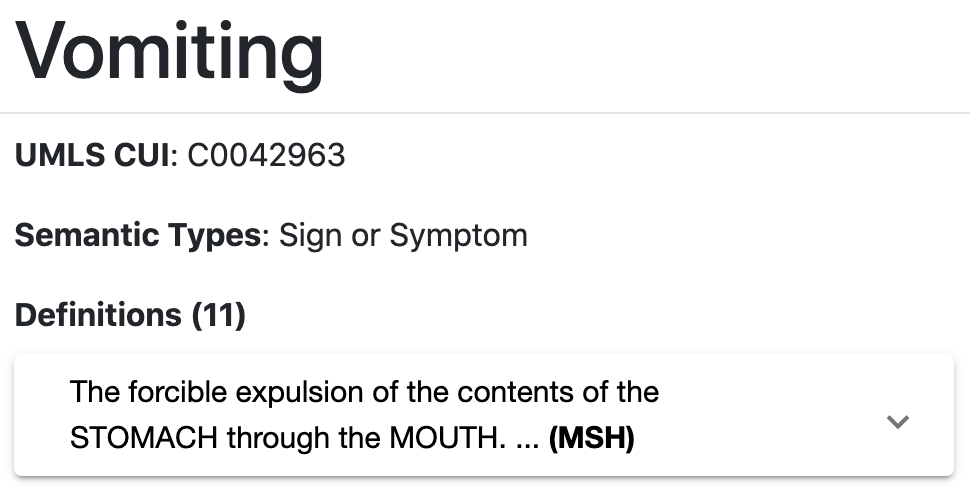
\includegraphics[width=0.45\textwidth]{umls-vomiting.png}}
  edge[ua-red,ultra thick,dotted,latex-] (vomiting);
\node[anchor=north, inner sep=0pt, below=3em of spinning]
  (umls-dizziness)
  {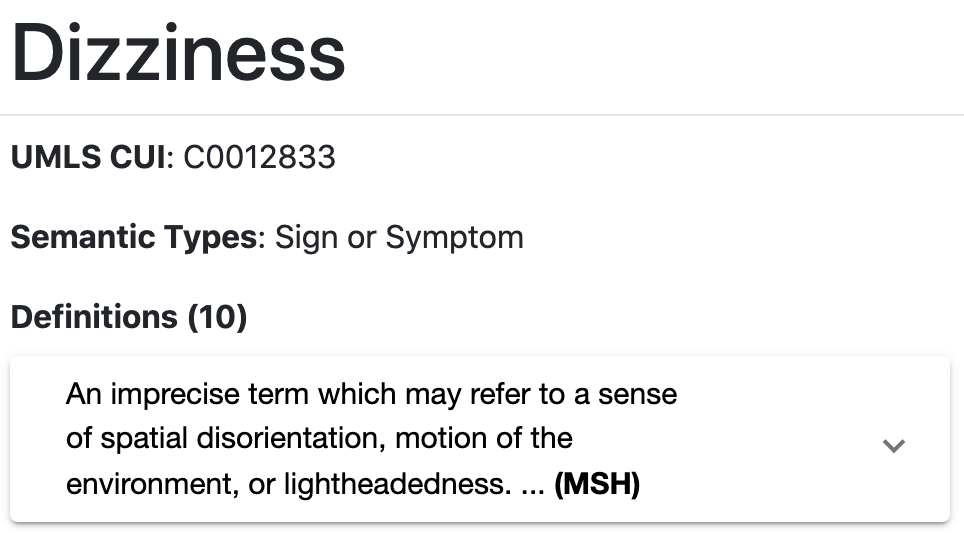
\includegraphics[width=0.45\textwidth]{umls-dizziness.png}}
  edge[ua-red,ultra thick,dotted,latex-] (spinning);
\node[draw,fit=(umls-vomiting) (umls-dizziness), inner sep=1em, label=below:{Unified Medical Language System (UMLS)}] {};
\end{tikzpicture}
}
\end{frame}

\begin{frame}{Normalization as vector-space search}
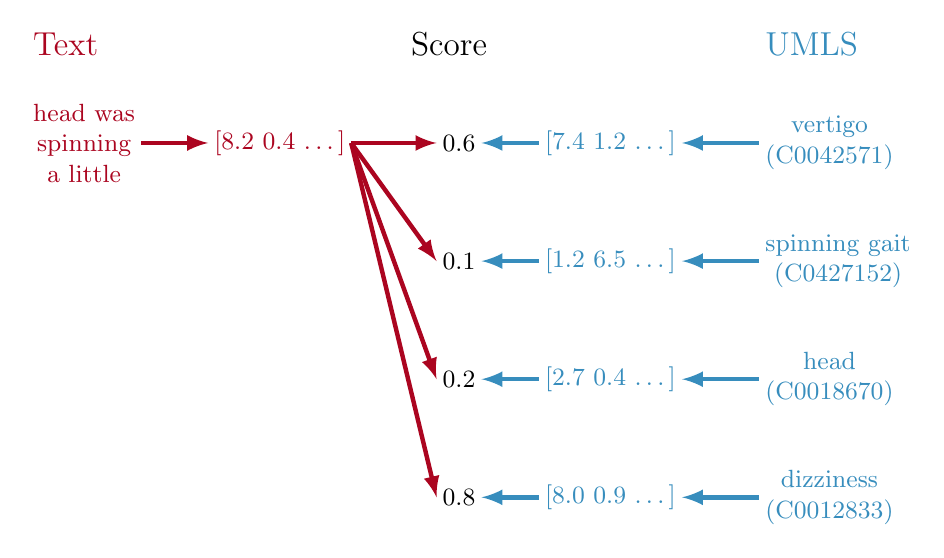
\begin{tikzpicture}[font=\small, inner sep=2pt, anchor=west]
\pgfmathsetseed{42}

\node[ua-red] at (0, 1.25) {\large Text};
\node<4-> at (4.8, 1.25) {\large Score};
\node[ua-oasis] at (9.3, 1.25) {\large UMLS};

\node[align=center,ua-red] (text) at (0, 0) {head was \\ spinning \\ a little};
\node<2->[ua-red] (text-vec) at (2.3, 0) {\small[8.2 0.4 \ldots]}
  edge[ua-red, ultra thick, latex-] (text);
\foreach[count=\i from 0, count=\slide from 4] \term/\vec/\score in {
    vertigo\\(C0042571)/[7.4 1.2 \ldots]/0.6,
    spinning gait\\(C0427152)/[1.2 6.5 \ldots]/0.1,
    head\\(C0018670)/[2.7 0.4 \ldots]/0.2,
    dizziness\\(C0012833)/[8.0 0.9 \ldots]/0.8} {
  \node[ua-oasis, align=center] (umls-\i) at (9.3, -1.5*\i) {\term};
  \node<3->[ua-oasis] (umls-vec-\i) at (6.5, -1.5*\i) {\vec}
    edge[ua-oasis, ultra thick, latex-] (umls-\i);
  \node<\slide-> (score-\i) at (5.2, -1.5*\i) {\score}
    edge[ua-oasis, ultra thick, latex-] (umls-vec-\i);
  \draw<\slide->[ua-red, ultra thick, -latex] (text-vec.east) -- (score-\i.west);
}
\end{tikzpicture}
\end{frame}

\begin{frame}{Triplet training a vector-space transformer}
Goal: train a term-to-vector network using UMLS

Approach:
\begin{itemize}
\item Create triplets of input term $t_i$, match $t_p$, mis-match $t_n$
\item Train network so $t_i$ is more similar to $t_p$ than $t_n$
\end{itemize}

\pause
\centering
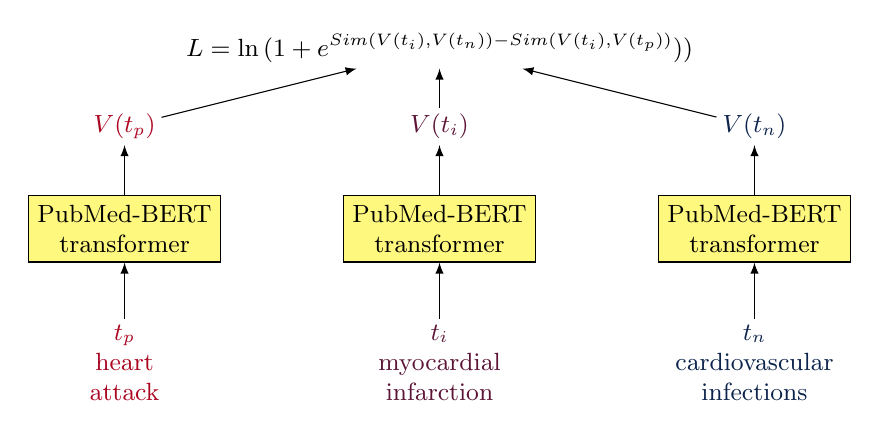
\begin{tikzpicture}[font=\small, text only/.style={inner sep=2pt, align=center}]
\node[text only]
  (L)
  at (0, 4)
  {$L = \ln{(1 + e^{Sim(V(t_i), V(t_{n})) - Sim(V(t_i), V(t_{p}))} )})$};
\foreach \i/\name/\textcolor/\phrase in {
    -4/p/ua-red/heart\\attack,
    0/i/ua-red!50!ua-blue/myocardial\\infarction,
    4/n/ua-blue/cardiovascular\\infections} {
  \node[text only, text=\textcolor]
    (input-\name)
    at (\i, 0)
    {$t_{\name}$ \\ \phrase};
  \node[draw, align=center, fill=yellow, fill opacity=0.5, text opacity=1]
    (bert-\name)
    at (\i, 1.7)
    {PubMed-BERT\\transformer}
    edge[latex-] (input-\name);
  \node[text only,text=\textcolor]
    (repr-\name)
    at (\i, 3)
    {$V(t_{\name})$}
    edge[latex-] (bert-\name)
    edge[-latex] (L);
}
\end{tikzpicture}
\end{frame}

\begin{frame}{Domain adaptation without retraining}
Adding new target domain terms for UMLS concepts:
\begin{itemize}
\item<3-> Encode terms with trained term-to-vector network
\item<4-> Search over these vectors just like UMLS vectors
\item<5-> No retraining necessary!
\end{itemize}
\medskip

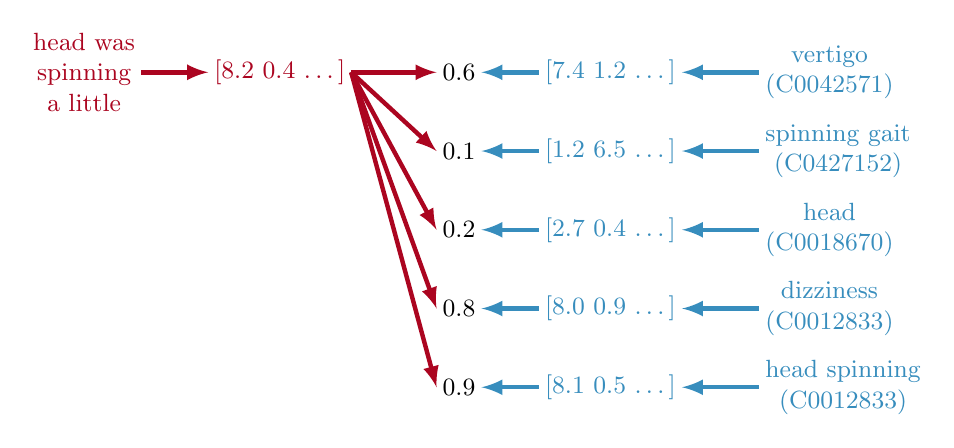
\begin{tikzpicture}[font=\small, inner sep=2pt, anchor=west]
\node[align=center,ua-red] (text) at (0, 0) {head was \\ spinning \\ a little};
\node[ua-red] (text-vec) at (2.3, 0) {\small[8.2 0.4 \ldots]}
  edge[ua-red, ultra thick, latex-] (text);
\foreach[count=\i from 0] \term/\vec/\score in {
    vertigo\\(C0042571)/[7.4 1.2 \ldots]/0.6,
    spinning gait\\(C0427152)/[1.2 6.5 \ldots]/0.1,
    head\\(C0018670)/[2.7 0.4 \ldots]/0.2/,
    dizziness\\(C0012833)/[8.0 0.9 \ldots]/0.8/} {
  \node[ua-oasis, align=center] (umls-\i) at (9.3, -\i) {\term};
  \node[ua-oasis] (umls-vec-\i) at (6.5, -\i) {\vec}
    edge[ua-oasis, ultra thick, latex-] (umls-\i);
  \node (score-\i) at (5.2, -\i) {\score}
    edge[ua-oasis, ultra thick, latex-] (umls-vec-\i);
  \draw[ua-red, ultra thick, -latex] (text-vec.east) -- (score-\i.west);
}
\visible<2->{
\node[ua-oasis, align=center] (umls-4) at (9.3, -4) {head spinning\\(C0012833)};
}
\node<3->[ua-oasis] (umls-vec-4) at (6.5, -4) {[8.1 0.5 \ldots]}
  edge[ua-oasis, ultra thick, latex-] (umls-4);
\node<4-> (score-4) at (5.2, -4) {0.9}
  edge[ua-oasis, ultra thick, latex-] (umls-vec-4);
\draw<4->[ua-red, ultra thick, -latex] (text-vec.east) -- (score-4.west);
\end{tikzpicture}
\end{frame}

\begin{frame}{Domain adaptation without retraining}
Evaluation data:
\begin{description}[NCBI]
\item[NCBI] disorders, MEDIC, PubMed abstracts
\item[B-D] diseases, MEDIC, BioCreative V challenge
\item[B-C] chemicals, CTD, BioCreative V challenge
\item[S/C] disorders, UMLS, ShARe/CLEF eHealth 2013
\item[MCN] various concepts, UMLS, 2019 n2c2 Shared-Task
\end{description}
\end{frame}

\begin{frame}{Domain adaptation without retraining}{}
{\small\centering
\begin{tabular}{ l c c c c c c}
\toprule
Approach & NCBI & B-D & B-C  & S/C & MCN \\
\midrule
PMB & \alert<2>{76.6}  & \alert<2>{76.7} & \alert<2>{91.8}  & \alert<2>{73.6}  & \alert<2>{60.0} \\
PMB + Train:O & \alert<2>{82.6}  & \alert<2>{84.4} & \alert<2>{95.8} & \alert<2>{83.5} &  \alert<2>{69.6}  \\
PMB + Train:O + Search:T & \alert<3>{89.5} & \alert<3>{92.3} & \alert<3>{96.7} & \alert<3>{89.2} &  \alert<3>{82.2}  \\
PMB + train per dataset & \alert<3>{91.2}  & \alert<3>{92.8}  & \alert<3>{96.9} & \alert<3>{90.4} & \alert<3>{83.7}  \\
%Previous state-of-the-art & 91.1 & 93.2 & 96.6 & 91.1 & 83.6 \\
\bottomrule
\end{tabular}

PMB = PubMedBERT; O = Ontology; T = target domain terms

}

Findings:
\begin{itemize}
\item<2-> Triplet-training on ontology yields better term-to-vector network
\item<3-> Adding new domain terms during search is nearly as good as retraining for each dataset
\end{itemize}
\end{frame}

\section*{Summary and future work}

\begin{frame}{Summary and future directions}
\begin{itemize}
\item Most domain adaptation work assumes access to source domain data
\item In the clinical domain, often only a model can be distributed
\item SemEval-2021 Task 10 established a new paradigm for evaluating domain adaptation
\pause
\item Initial promising approaches:
\begin{itemize}
\item Source-free self-training for negation detection
\item Source-free active-learning for time expression recognition
\item Source-free term-to-vector networks for concept normalization
\end{itemize}
\end{itemize}
\end{frame}


\begin{frame}{Collaborators}
\centering

\begin{block}{University of Arizona}
\begin{tabular}{c c c c }
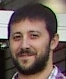
\includegraphics[height=0.2\textheight]{Egoitz.jpg} &

\includegraphics[height=0.2\textheight]{Xin.jpg} &
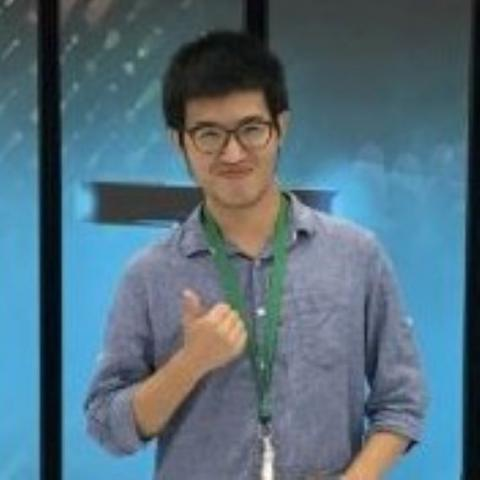
\includegraphics[height=0.2\textheight]{Dongfang.jpg} &
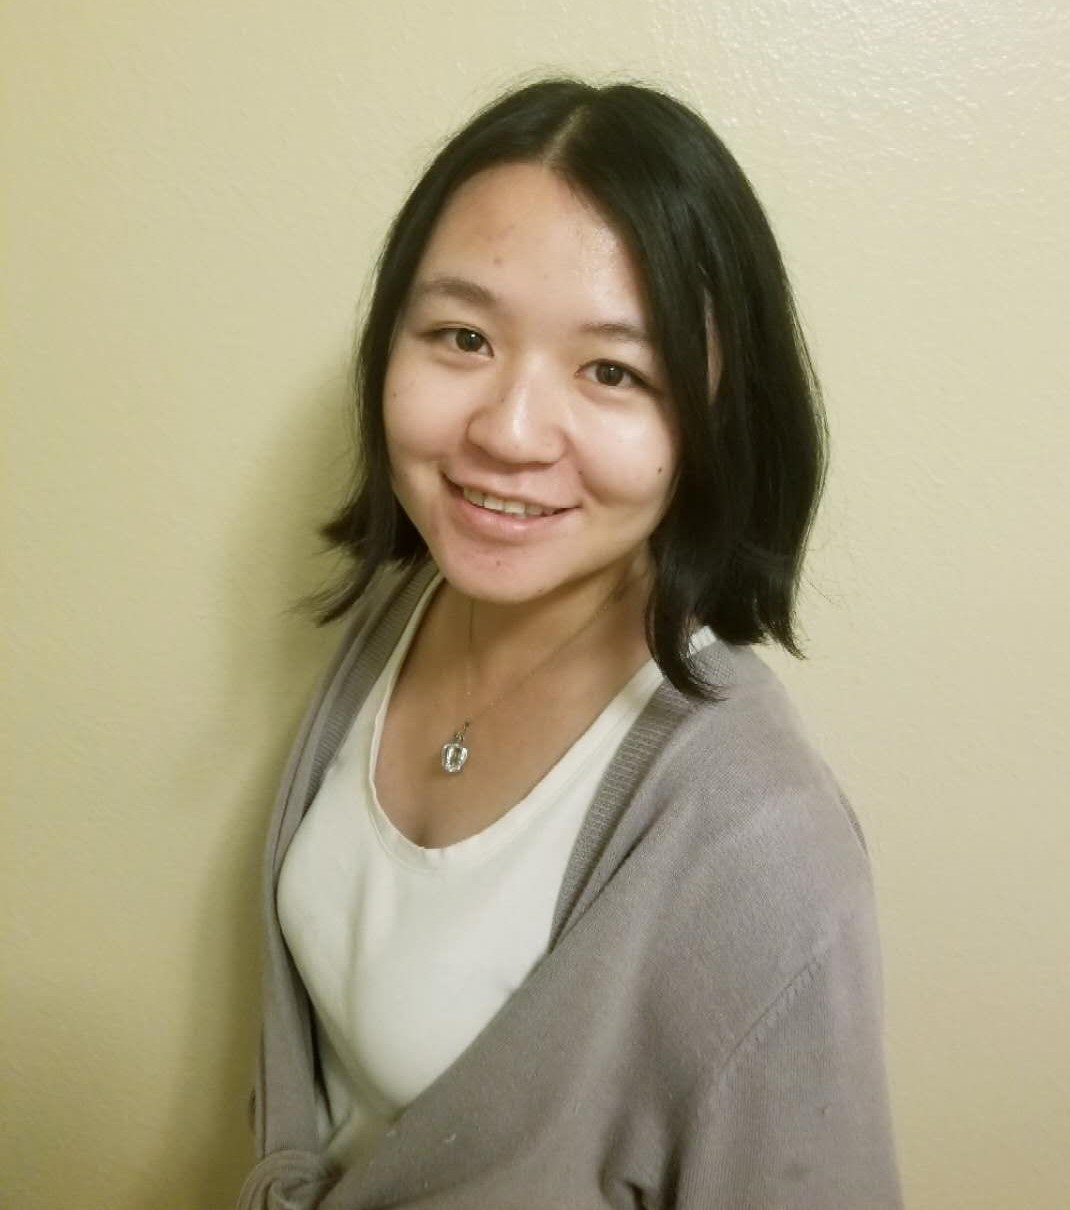
\includegraphics[height=0.2\textheight]{Yiyun.jpg} \\
Egoitz Laparra & Xin Su & Dongfang Xu & Yiyun Zhao
\end{tabular}
\end{block}

\begin{block}{Harvard / Boston Children's Hospital}
\centering
\begin{tabular}{c @{\hspace{5em}} c}
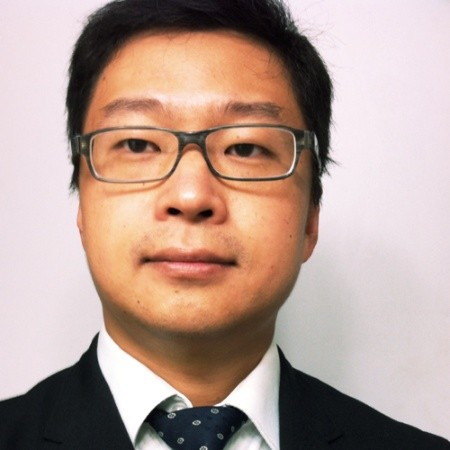
\includegraphics[height=0.2\textheight]{Chen.jpeg} &
 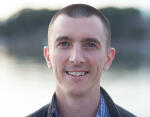
\includegraphics[height=0.2\textheight]{Tim.jpg} \\
Chen Lin & Tim Miller
\end{tabular}
\end{block}
\end{frame}

\appendix

\begin{frame}[allowframebreaks]{References}
\scriptsize
\bibliographystyle{apalike}
\bibliography{domain-adaptation.bib}
\end{frame}


\end{document}
